%# -*- coding: utf-8-unix -*-
% !TEX program = xelatex
% !TEX root = ../thesis.tex
% !TEX encoding = UTF-8 Unicode


\chapter{跨语言的表格实体链接研究}
\label{chap:tabel}

本章研究的实体链接任务中,待链接文本为以源语言编写的互联网表格,
而知识库则以目标语言编写,因此我们将其称为跨语言的表格实体链接。
为了捕捉不同于传统实体链接任务的特性,
我们提出了基于神经网络和跨语言词向量的表格链接模型,
旨在让不同语言的连续特征空间得以兼容,并捕捉表格具有的多种粒度的匹配特征。
%在中英文跨语言表格链接实验中,本章提出的模型


%This paper studies the problem of linking string mentions from web tables in one language
%to the corresponding named entities in a knowledge base written in another language, 
%which we call the cross-lingual table linking task. 
%We present a joint statistical model to simultaneously link all mentions that appear in one table.
%The framework is based on neural networks, aiming to bridge the language gap by 
%vector space transformation and a coherence feature that captures the correlations 
%between entities in one table.
%%Experimental results show that our approach outperforms all baseline methods by a relative gain of 12.1\%,
%Experimental results report that our approach improves the accuracy of cross-lingual table linking
%by a relative gain of 12.1\%.
%Detailed analysis of our approach also shows a positive and important gain
%brought by the joint framework and coherence feature.~\footnote{Kenny Q. Zhu
%is the contact author. This work was supported by NSFC grant No. 
%91646205 and 61373031, as well as SJTU funding project 16JCCS08.}

%# -*- coding: utf-8-unix -*-
% !TEX program = xelatex
% !TEX root = ../thesis.tex
% !TEX encoding = UTF-8 Unicode

\section{概述}%intro
\label{sec:tabel-intro}

% basic introduction to table linking

海量的互联网文本信息中,充斥着以HTML编写的表格,
即互联网表格\cite{cafarella2008webtables,wang2012understanding}。
和纯文本相比,互联网表格中的行列形式携带了非常有价值的结构化信息。
为了能让机器理解,并且很好的处理表格中的信息,%~\parencite{wang2012understanding},
第一个步骤就是需要识别每个单元格中文本内容所对应的实体,
并映射到一个标准词库,或是知识库上,例如维基百科或Freebase。
这样的一个在互联网表格上进行实体链接的任务,
在本章节被称为表格链接\cite{bhagavatula2015tabel,wu2016entity}。

对于表格链接任务,
已有的研究工作\cite{bhagavatula2015tabel,limaye2010annotating}主要针对英文表格,
由于使用知识库也为英文,表格链接是在单一语言场景中进行的。
然而,当需要链接的表格以其它语言编写的时候,
对应语言的非英文知识库往往不够全面,无法涵盖目标表格中提及的所有实体。
例如中文版维基百科,其中包含的实体(页面)数量仅为英文维基百科的1/6左右。
%多聊几句?
基于不同语言知识库大小上的差异,
本章探寻一种全新的方式将非英文表格与英文知识库相连,
该任务也被称为\textbf{跨语言表格链接}。
如\figref{fig:tabel-intro}所示,
中文表格里的电影 ``{邮差}'' 在中文维基百科里没有对应的实体,
但存在对应的英文维基实体 ``Il Postino: The Postman'' ,
因此可以建立跨语言的链接。

\begin{figure}[th]
\centering
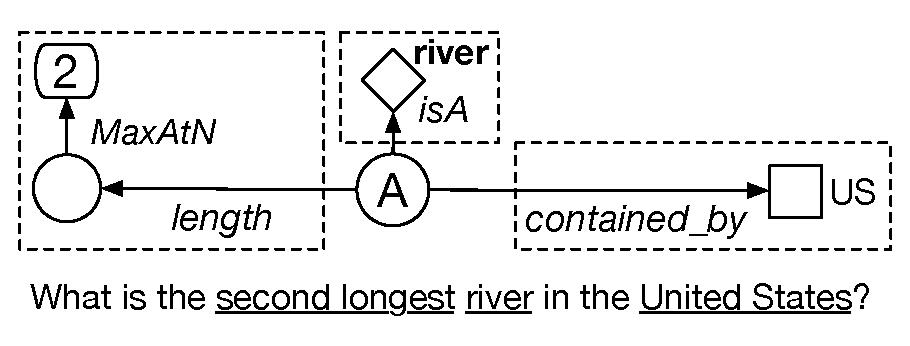
\includegraphics[width=0.9\columnwidth]{figure/tabel/intro.eps}
%\scalebox{0.22}{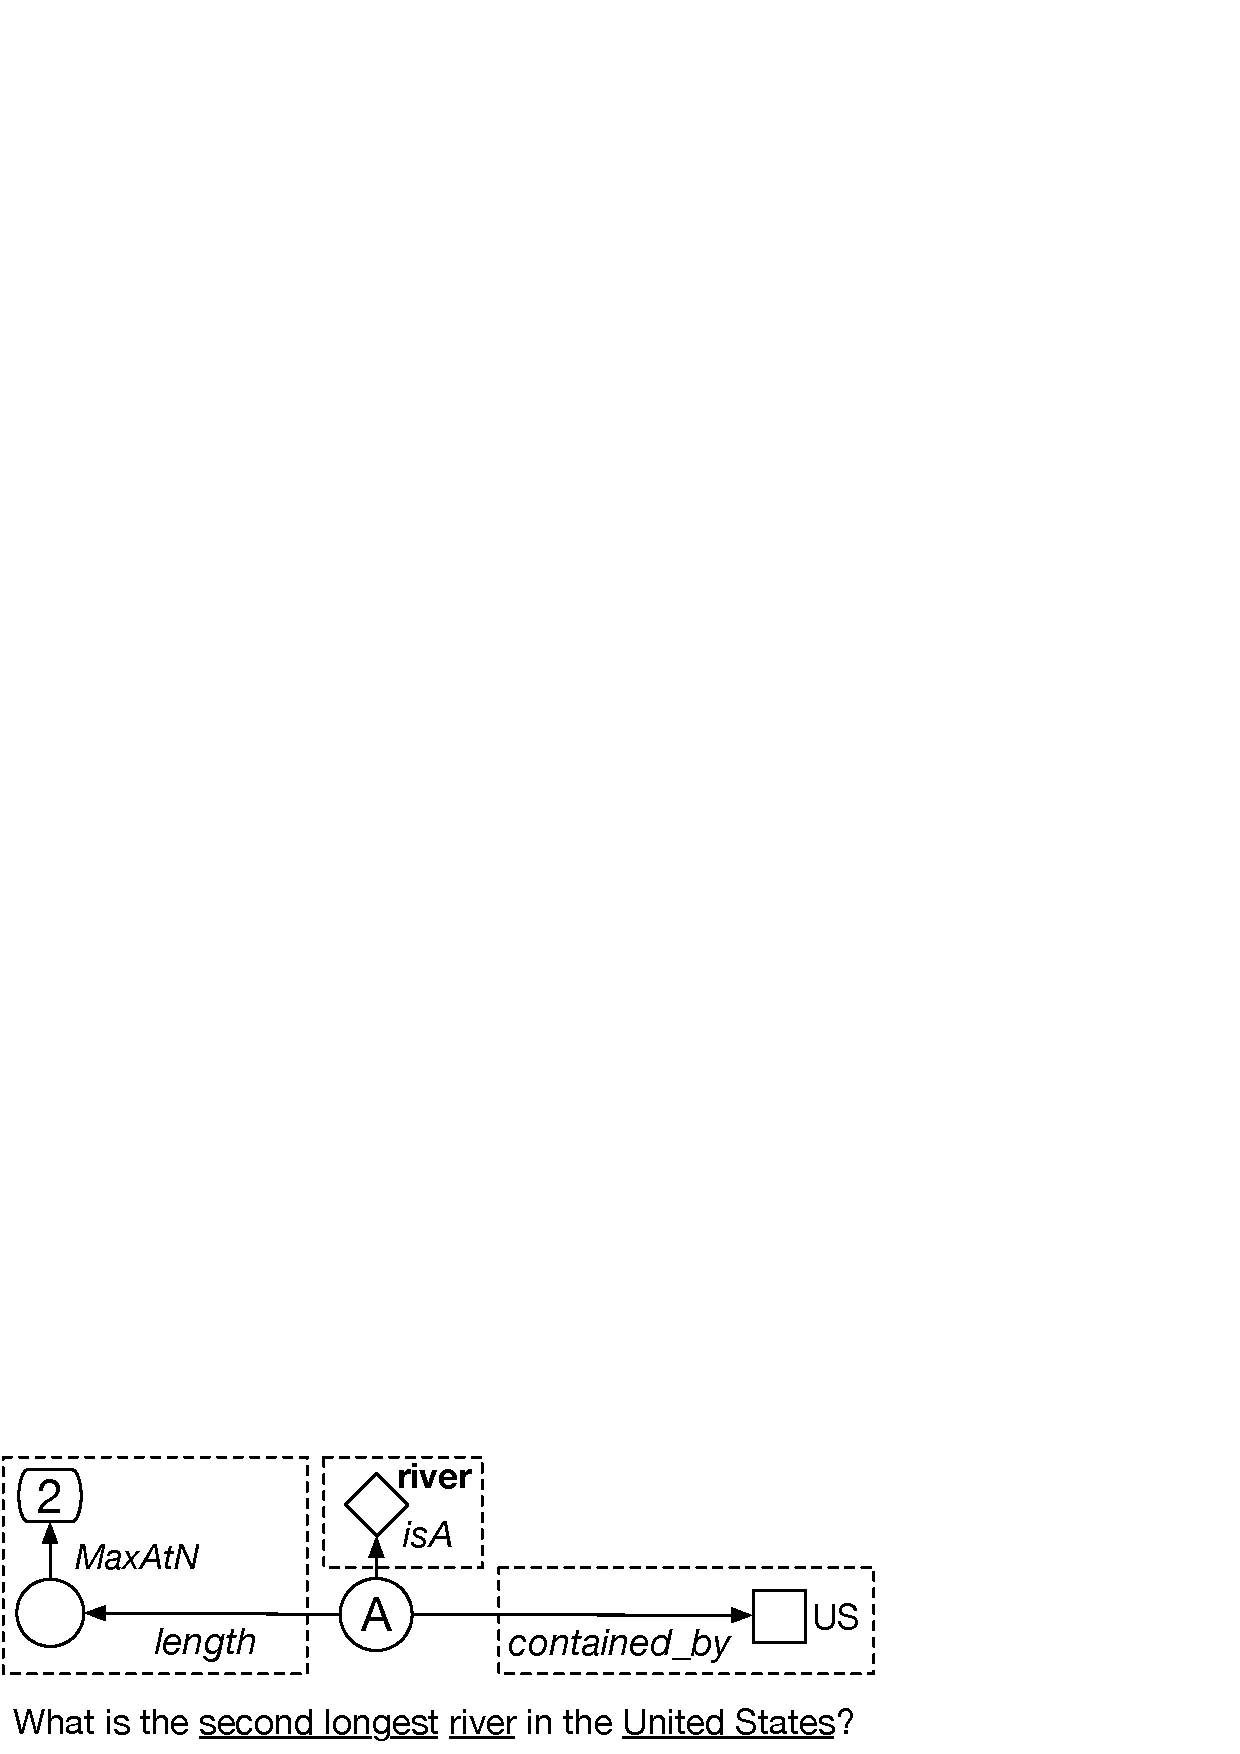
\includegraphics[angle=0]{figure/tabel/intro.pdf}}
\bicaption{中文表格到英文知识库的跨语言链接示例。}
{Example of cross-lingual table linking from Chinese to English.}
\label{fig:tabel-intro}
\end{figure}

帮助目标知识库补充事实三元组,是我们尝试跨语言表格链接的另一个动机。
英文知识库比其它语言知识库更加庞大,也更加结构化,但仍然包含许多长尾实体。
这些实体仅出现知识库的极少数事实三元组中,例如别国的电影、名人等,
考虑到英文知识库的贡献者更多以英语为母语,这些实体的相关信息就很容易被忽略。
另一方面,海量非英文的互联网表格成为了与长尾实体相关的丰富的语义信息来源。
例如,\figref{fig:tabel-intro}描述了电影与它的原产国之间的关系。
国产电影 ``{线人}'' 有对应的英文维基页面 ``The\_Stool\_Piegon\_(2010\_film)'' ,
但与之相应的Freebase实体却缺少许多相关的知识。
若我们准确将该电影链接至维基百科,
并根据表格前两列的多个实体对推理出关系$film\_country$,
那么就可为知识库补充新的事实。

%In this paper, we attempt to solve the cross-lingual table linking problem
%{\em without} using any non-English knowledge bases.
%%That is, our goal is to link the mentions in the non-English table 
%%directly to an entity in the English knowledge base. 
%%The advantage of this is we do not discard any information of non-English mentions
%%so that our model has the ability to tolerate the error caused by translation.
%To the best of our knowledge, this is the first attempt that attacks the 
%cross-lingual table linking problem. 


具体论述我们提出的跨语言表格链接方法之前,首先来讨论两种朴素的做法。
第一种方式主要基于已有单一语言的表格链接技术,
将表格映射到语言一致的非英文知识库,
然后再利用知识库之间存在的跨语言链接,%~\parencite{tsai2016cross},
将实体翻译至英文知识库。
例如不同语言的维基百科之间就存在着人工编辑好的跨语言链接。
这种方式的主要问题在于:
1) 非英文知识库的信息量较低,可能无法覆盖每一个单元格的实体;
2) 并不是每个非英文知识库都会存在和跨语言链接。

第二种做法中,整个非英文表格的内容首先直接被翻译成英文,
然后整个问题便退化成英文上的表格链接,以往方法可以直接套用。%\parencite{mcnamee2011cross}。
%这种两阶段方式依然不够有效,
它与远距离监督模型很相似,各单元格的(非英文名称,英文实体)对并不直接作为训练数据。
%翻译过程的错误会被传播到之后的链接步骤,而无法得到反馈。
此法的缺陷在于对已有翻译工具准确率的高度依赖:
一方面,文本翻译过程仅生成单一结果,一旦错误则对后续链接步骤影响很大;
另一方面,翻译工具如同黑盒,无法根据训练数据进行优化。

在本章中,为了使研究具有普适性,我们忽略不同语言知识库之间的跨语言链接,
尝试在\textbf{不使用}任何非英文知识库进行过渡的情况下,解决跨语言的表格链接任务。
据我们所知,本章节提出的解决方案,是对跨语言表格链接的第一次尝试。

对于实体链接任务而言,
%\parencite{tsai2016cross,mcnamee2011cross,bhagavatula2015tabel,wu2016entity},
无论是否跨语言,第一个步骤总是为每个单元格生成一组候选实体,
之后整个任务转换为排序问题,对每单元格寻找与其描述最接近的候选实体。
主要的技术挑战在于表格描述和知识库来自不同的语言,
无法依靠任何字面上的相似特征。
此外,表格中缺少纯文本里的谓语、状语等相关上下文,
给单个实体的消歧义带来了困难。
%The major technical challenge of our task is since the source mention
%and the target entity come from two different languages,
%their feature representations are naturally incompatible. 
%To make matters worse, tables offer very limited context for disambiguating
%a mention in the first place.

%Since the language of source mention and target entity is inconsistent, 
%it's hard to direct use the surrounding infomation of them \XS{rephrase}. 
%Besides, this task still has to face a lack of surrounding contexts 
%which can be very helpful during entity disambiguation in normal entity linking tasks.

% image CNN, table is like image

为了解决上述的两个挑战,
我们提出了基于神经网络的联合模型来解决跨语言表格链接问题,
它具有以下三个特点。
首先,模型主体基于跨语言词向量,我们将单元格的描述短语、%mention
上下文、以及知识库的实体映射到不同语言对应的连续向量空间作为语义特征表示,
并且使用线性变换的方式,实现不同语言的向量空间统一。
其次,模型充分利用表格中同一行列的实体所具有的相关性,
并通过神经网络学习不同粒度的相关性特征。
最后,模型基于联合训练思路,以优化整张表格的匹配程度作为目标函数,
使用成对排序损失函数进行参数学习以及多轮迭代的预测方式,对新的表格完成链接。

%Most existing work \XS{cite} mines hand-crafted features to measure the similarity 
%between mentions and candidate entities.  Since feature engineering suffers XXX, 
%some work attempt to use nerual network \XS{cite} to generate fearures, 
%which shows great improvements in task of entity linking. 
%
%As we should notice, a table can be regarded as a matrix of texts, similar to an image, which is a matrix of pixels. 
%Inspired by that idea of using deep neural networks to capture rich semantics of images, which has been proven successful, 
%we present a jointly modeling framework based on nerual networks to solve our problem.
%Besides, Convolotional Neural Networks(CNN) is a natural structure to deal with data in matrix form such as tables.

% Contribution
本章的贡献可以总结为以下四个部分:
\begin{enumerate}
\item{我们首次尝试在跨语言场景上进行表格链接;}
\item{我们提出了一个基于神经网络的联合训练模型,能有效捕捉原始表格与候选链接表格的语义相关性,
并消除不同语言之间的语义间隔;}%这一段写的很烂,可能要改
\item{联合模型除了捕捉单个单元格描述与候选实体间的语义关联特征,
还提出了一种一致性特征,用于捕捉候选链接表格内部不同实体间的联系,有效提升模型的预测准确率;}
\item{我们构建了从中文到英文的跨语言表格链接数据集用于实验,
本章提出的模型效果显著优于其它基线模型,
同时我们进行了一系列分析实验,以验证模型各部分的有效性。}
\end{enumerate}

%\begin{itemize}
%\item We are the first to define the problem of cross-lingual entity linking 
%for web tables (\secref{sec:problem});
%\item We present a novel neural network based joint model which effectively captures the rich semantics of mention table and referent entity table simultaneously. Based on that, we bridge the gap between different languages in this task (\secref{sec:translation} and \secref{sec:cell});
%\item We propose a coherence feature in the joint linking model which captures the correlation of entities appearing in the same table and improves the linking accuracy (\secref{sec:coherence});
%\item The framework significantly outperforms
%several baseline methods, with an accuracy of 62.9\%. (\secref{sec:eval}).
%%and question answering. Furthermore, our schema representation is
%%on par with the popular word embedding model in computing relation similarity (\secref{sec:eval}).
%\end{itemize}

%# -*- coding: utf-8-unix -*-
% !TEX program = xelatex
% !TEX root = ../thesis.tex
% !TEX encoding = UTF-8 Unicode

\section{相关工作}%related
\label{sec:tabel-related}

% %\label{sec:el}
% Entity linking has been a popular topic in NLP for a long time as it is the basic step for machines to understand natural language and an important procedure of many complex NLP applications such as information retrieval and question answering. Entity linking requires a knowledge base to which entity mentions can be linked, the most popular ones including Freebase~\cite{bollacker2008freebase}, YAGO~\cite{suchanek2007yago} and Wikipedia~\cite{cai2013wikification}, where each Wikipedia article is considered as an entity. 
% %Most works focus on linking to Wikipedia and thus the task is also named as Wikification. The typical procedure of entity linking contains two stages: candidate generation, where the surface forms (mention) in the query text which could be linked to certain entities in the KB are identified, and a set of candidate entities are proposed for each entity mention; candidate ranking, where the candidates for each mention are ranked (usually based on context) and the best one is returned as linking result. 
% Due to its fundamental role in many applications, the task of entity linking has attracted a lot of attention, and many shared tasks have been proposed to promote this study~\cite{ji2010overview,cano2014microposts2014,carmel2014erd}.
% %Wikipedia was first explored by Bunescu and Pasca~\cite{pasca2006using}, where an SVM kernel was used to compare the lexical context of an entity mention to each candidate's Wikipedia page. Since each entity mention needed to train its own SVM model, the experiment was limited. Later, Mihalcea and Csomai~\cite{mihalcea2007wikify!:} proposed a system called Wikify! for the Wikification task. They applied word sense disambiguation to this task, and experimented with two methods to link detected candidates to a Wikipedia page: 1) comparing the mention's lexical context to content of disambiguation page; 2) training a Naive Bayes classifier for each ambiguous mention. 
% %Later approaches made use of the observation that entity disambiguation in the same document should be related. Cucerzan~\cite{cucerzan2007large-scale} maximized the agreement between the context data stored for each candidate entity and the contextual information in the document, and also the agreement among the category tags of the candidate entities. Milne and Witten~\cite{milne2008learning} took a similar approach but relied on unambiguous terms in the context. Han and Zhao~\cite{han2009named} constructed a large-scale semantic network from Wikipedia, then computed similarity between query and candidate entity based on the semantic network. Ratinov et al.~\cite{ratinov2011local} formalized this task into a bipartite graph matching problem and proposed a score function which considered both local similarity and global coherence. Zhang et al.~\cite{zhang2011wikipedia} employed a Wikipedia-LDA model and the contexts were modeled as a probability distribution of Wikipedia categories. The similarity score between candidates and entities were computed based on the category distribution. 
% %Cai et al.~\cite{cai2013wikification} proposed to first enrich the sparsely-linked articles by adding more links iteratively and then use the resulting link co-occurrence matrix to disambiguate the mentions in an input document. Yang and Chang~\cite{yang2016s-mart:} proposed a tree-based structured learning framework, S-MART, which is particular suitable for short texts such as tweets. 
% 

对互联网表格的研究最早开始于Cafarella等人的工作\cite{cafarella2008webtables},
文中指出大约有1.54亿表格可以作为高质量的关系数据源。
例如文献\parencite{munoz2014using,sekhavat2014knowledge}关注于从表格中寻找
不同列之间的关系,从而实现向知识库中补充新的三元组。
这些工作都假定实体链接已完成,而若要对更广范围的表格数据进行关系挖掘,
表格链接始终是其前置步骤,链接准度直接决定了后续步骤的质量。
%如概述中指出,  表格关系可以补充三元组
%Munoz:找关系 挖掘不同行之间,但是是同样的两列之间的实体关系,映射至DBPedia 构成三元组,即挖掘语义。  并补充缺失
%在维基百科内部(已有链接)
%按已有match比例尝试一些predicate,然后学习一个triple是对还是错
%Sekhavat: Tabular KBC 同样是假设linking已好的情况 利用PATTY作为跳板,根据EP之间存在的pattern,寻找到rel的关系
%条件概率  (相当于EP有一系列的外部文本pattern,而不是仅有KB)
%rel来自YAGO
%(Fuck...但两者根本都是column-column-rel和predicate的一一对应)

和纯文本上的实体链接任务不同,表格文本上的链接聚焦于表格中的每一个单元格,
并且对于任何一个待链接的单元格,其它同行或同列的单元格与其有着更加密切的语义联系。
%不同的研究工如何利用好表格的半结构化
%如何利用同行列实体间的关联
目前已有的表格链接研究主要基于特征工程。
Limaye等人\cite{limaye2010annotating} 以YAGO为知识库,解决更加宽泛的表格链接任务,
包括将单元格链接至实体、列头链接至类型,以及两列之间的关系链接至谓词,
同时创建了WebManual数据集。
作者提出了一个概率图模型用于同时完成不同的链接子任务,
并通过人为定义的多种势函数表示单元格、实体、类型、谓词语间的组合特征,
整个表格链接的目标函数为多种势函数的连乘,不同子任务的决策互相影响,
使得模型在捕捉单个单元格与实体相匹配的同时,也能兼顾实体与列头类型的一致性,
以及不同列实体间与特定谓词的相关性。
%全局优化
%概率图模型,定义了potential,用于描述pair或这triple feature among type,entity,relation
%都是feature indicator
%1. cell vs entity (tfidf-cos, jaccard, soft-cos ...)
%2. header vs type (the same)
%3. entity vs type (e \in T)
%4. type vs rel (soft schema match)
%5. entity vs rel
%特征都比较直观简单,but,
%Experiments show that attacking the
%three subproblems collectively and in a unified graphical inference
%framework give clear accuracy benefits compared to
%making local decisions
Bhagavatula等人\cite{bhagavatula2015tabel}利用了表格上下文的词汇信息,
对于待链接的单元格,将其行或列方向上的其它单元格文本合并形成上下文词袋,
与候选实体所对应的词汇进行相似度计算,得到多个相似度特征用于模型训练,
并采用迭代更新方式进行预测。
%graph model,iterative update配上features
%每个cell确定了context之后独立计算
%上下文特征(word level,entity level)
%coherence(MW)
Wu等人\cite{wu2016entity}首次尝试对中文表格进行链接,
提出的模型首先构建由单元格和所有候选实体组成的连通图,
然后在图中进行类似PageRank算法\cite{page1999pagerank}
的随机游走,以选择最佳链接结果,因此是一种非监督学习方式。
候选实体是否同行列决定了图中是否存在直接相连的边,
而单元格与实体、实体与实体之间所连边的权重则由预定义的相似度公式计算,
使用了编辑距离、词袋相似度、实体于三元组中共现等特征。
区别与以上研究,本文的工作基于深度学习,尝试不依赖常用的相似度计算公式,
而是利用神经网络挖掘表格和目标实体在多个粒度上的特征。


% %\subsection{Cross-Lingual Entity Linking}
% %\label{sec:cl}
% Starting from 2011 the annual TAC KBP Entity Linking Track has been using the multi-language setting~\cite{ji2010overview,ji2014overview,ji2015overview}, where the languages involved are English, Chinese and Spanish. 
% %Most systems for this task were adaptations of mono-lingual entity linking systems: either first do entity linking on foreign languages and then translate the results to English via language links, which requires a comprehensive knowledge base in the foreign languages; or first translate the query into English by some machine translation tool and then apply English entity linking algorithms, whose performance greatly relies on the machine translator. 
% %Some other systems tried to avoid the usage of such assumptions. McNamee et al.~\cite{mcnamee2011cross} first experimented with cross-lingual entity linking on documents. They first used a machine translation tool developed by Irvine et al.~\cite{irvine2010transliterating} to transliterate the detected query mentions into English and transform the task into a mono-lingual one. Then they extracted some features and ranked the candidates with SVM-rank. However, to train this model, parallel corporas which are well aligned at sentence level are required.
% Most methods managed to bridge the language gap through language-independent spaces.
% Fahrni et al.~\shortcite{fahrni2011hits} presented HITS' system for cross-lingual entity linking. Their approach consisted of three steps: 1) obtain a language-independent concept-based representation for query documents; 2) disambiguate the entities using an SVM and a graph-based approach; 3) cluster the remaining mentions which were not assigned any KB entity in step 2.
% Zhang et al.~\shortcite{zhang2011wikipedia} leveraged a modified version of Latent Dirichlet Allocation, which they call BLDA (Bilingual LDA) and bridged the gap between languages via topic space. 
% %They trained the topic model on English-Chinese Wikipedia page pairs (indicated by inter-language links) and disambiguated candidate entities by computing the inner product of the topic distributions of the query text and the entity Wikipedia page. Their approach does not require supervised learning and performs well with a conservative candidate generation stage. 
% Wang et al.~\shortcite{wang2015language} proposed an unsupervised graph-based method which matches a knowledge graph with a graph constructed from mentions and the corresponding candidates of the query document.
% Tsai et al.~\shortcite{tsai2016cross} trained a multilingual word and title embeddings and ranked entity candidates using features based on these multilingual embeddings. 
% %They used canonical correlation analysis~\cite{hotelling1936relations} to project the embeddings of two languages into the same space, whose goal is the same as the translation layer in our model.


跨语言的实体链接的主要目的是将文本中的实体短语链接至另一个语言构建的知识库上,
近几年的TAC-KBP数据集\cite{ji2010overview,cano2014microposts2014,carmel2014erd}
中包含了跨语言的实体链接任务。
%以2015年的TAC-KBP任务为例,
%%Ji: Overview of the TAC-KBP2015 entity discovery and linking tasks 数据集
%目标知识库为英文维基百科,待链接的纯文本则来自英语、汉语、西班牙语这三种语言。
%相对于英文而言,其它语言下的知识库较为匮乏,
%因此跨语言实体链接的意义在于借助信息量更大的英文知识库,
%更好地理解外文文本中的信息。
为了解决此类问题,%跨语言场景中的实体链接任务,
McNamee等人\cite{mcnamee2011cross}提出了一种基线方法,
利用已有的翻译工具将外文文本转换为英语,
再使用传统的单语言链接模型完成任务。
%这样的方法,好处在于模型简单易于实现,
%但同时也具有一个很大的缺陷,就是
%此法的缺陷在于对已有翻译工具准确率的高度依赖:
%一方面,文本翻译过程仅生成单一结果,一旦错误则对后续链接步骤影响很大;
%另一方面,翻译工具如同黑盒,无法根据训练数据进行优化。
%TODO:后续如果有时间,可以聊聊cross-lingual word embedding,但肯定不是限制该干的事情。
为了尽可能减少对翻译工具的高度依赖,
模型需要能学习同一个实体或概念在不同语言下的抽象表达,
并通过特定运算体现出不同抽象表达之间的联系,以完成语义的跨语言兼容。

基于跨语言词向量的链接模型是一种可行的解决方案,
跨语言词向量的相关内容已在\secref{sec:rw-linking-cle}中介绍。
Tsai等人\cite{tsai2016cross}首先分别训练英文和外文的词向量,
再用典型相关分析(CCA)学习各自语言的转移矩阵,使得不同语言词向量位于同一连续空间,
之后依据该词向量计算短语和实体在不同粒度上下文中的余弦相似度,形成多个特征进行训练。
Sil等人\cite{sil2017neural}提出了更加复杂的深度学习模型,
以学习短语上下文和实体在句子级别和单词级别的相似特征,
同时在实验中比较了CCA、均方误差等多种生成跨语言词向量的方式。
%Sil 2016
%Wang
%fahrni
除了跨语言词向量以外,Zhang等人提出的跨语言主题模型\cite{zhang2013cross}
也可用于描述不同语言上的相同语义。
传统的LDA主题模型\cite{blei2003latent}旨在描述文档的语义表示,
通过对 ``{文档—主题}'' 与 ``{主题—单词}'' 间的概率进行建模,
将一个文档表示为抽象主题上的概率分布。
考虑到同一个实体在不同语言中的维基页面,
虽然单词不同,但其主题十分相似,
因此双语LDA模型中,同一个抽象主题对应不同语言上的两个``{主题-单词}'' 概率分布,
从而外语上下文和英语维基页面之间可以在主题层面上概率分布比较,实现链接过程。


本文的工作是表格链接和跨语言实体链接两者的综合体现,同时也是首次对此问题进行研究。

%# -*- coding: utf-8-unix -*-
% !TEX program = xelatex
% !TEX root = ../thesis.tex
% !TEX encoding = UTF-8 Unicode

\section{任务规范定义}
\label{sec:tabel-problem}

%The task of cross-lingual table linking: table info & entity info

%1. table info
%The task of cross-lingual table linking involves two kinds of information:
%mention tables and entities in the knowledge base.

输入的互联网表格$X$是一个具有$R$行和$C$列的矩阵,
每一个单元格$x_{ij}$的内容是由语言$L_1$(例如中文)描述的词语序列。
给定由另一种语言$L_2$(例如英文)编写,并包含大量实体$e$的知识库$K$,
跨语言表格链接的任务是寻找$X$对应的目标链接表格$E$,
使得链接表格中的每一个实体$e_{ij} \in K$对应单元格$x_{ij}$内容的消歧义表示。

在具体场景中,输入的表格包括一些无法被链接的单元格,
例如数字、日期、时间以及一些知识库中尚不存在的新兴实体。
一些已有工作\cite{ibrahim2016making}主要负责在互联网表格中识别这些数字或时间实体,
因此在本章中,我们不关注一个单元格是否能被链接的判断方式。
具体到任务定义中,
$P$为输入表格中所有可以被链接的单元格坐标$(i, j)$所构成的集合,
并且我们假设在训练集和测试集中,
每个输入表格$X$对应的可链接位置集合$P$都是已知的。

传统的实体链接方法通常在模型中定义一个评分函数$S(x, e)$,
用于衡量文本$x$与目标实体$e$之间的相关程度。
在表格链接任务中,这样的做法等同于将不同的单元格分割开,单独计算相似度。
然而缺陷在于,相邻或是同行列的目标实体之间的交互完全无法体现在链接模型中。
为了将目标链接表格中不同实体间的耦合关系融入任务中,
我们定义了在表格层面的评分函数,并以此预测最佳的链接表格$\hat{E}$,
如下所示:%TODO: argmax 显示错误
\begin{equation}
  \label{eqn:joint-score}
  \hat{E} = \argmax_{E \in GEN(X)} S(X,E),
\end{equation}
\noindent
其中$GEN(X)$表示由$X$生成的所有候选链接表格。
该函数描述了输入表格与候选实体表格之间的整体相关性分数。
%可以在这里扯joint和non-joint的区别。



%============================================================%

\section{我们的方法}
\label{sec:tabel-approach}

本节中,我们主要阐述使用联合训练模型解决跨语言表格链接的具体细节。
\figref{fig:tabel-overview}为整个模型的示意图。
之所以将整个模型成为 ``{联合训练模型}'' ,是因为神经网络的输入
包含了整个互联网表格$X$,以及对应的一个候选链接表格$E$,
而模型的输出代表两者的相关性分数$S(X, E)$。

具体而言:
1) 我们首先对表格中的每一个单元格内容生成一系列知识库中的候选实体;%(\secref{sec:candgen}),
2) 模型对单元格词组和实体进行向量编码,
并学习基于它们向量表示的\textbf{指示特征}以及\textbf{上下文特征};%(\secref{sec:cell}).
3) 为了使不同语言下的语义向量互相兼容,
模型利用双语翻译矩阵将向量表示从中文转为英文;%(\secref{sec:translation}).
4) 模型从候选表格$E$的内部学习第三类特征,即候选实体间的\textbf{一致性特征}。%(\secref{sec:coherence}).
%We combine these three features together to calculate the overall relevance score, and finally
本节最后将介绍训练和测试的具体流程,以及整个模型中重要的一些实现细节。%(\secref{sec:strategy}). 

\begin{figure*}
	\centering
	%\epsfig{file=figures/overview.eps, angle=0, width=2.0\columnwidth}
    \includegraphics[width=\columnwidth]{figure/tabel/overview.eps}
	\bicaption{基于神经网络的联合训练模型示意图。}{Overview of proposed neural network based joint model.}
	\label{fig:tabel-overview}
\end{figure*}

%# -*- coding: utf-8-unix -*-
% !TEX program = xelatex
% !TEX root = ../thesis.tex
% !TEX encoding = UTF-8 Unicode

\subsection{候选实体生成}
\label{sec:tabel-candgen}

%To generate the candidate entity table,

我们对中文表格$X$的每一个单元格内容生成一系列英文知识库中的候选实体。
在本章的研究中,我们使用英文维基百科作为知识库。
由于提出的方法不使用任何中文知识库进行过渡,
为了实现语言转换,我们首先利用已有的翻译工具生成中文词组对应的多种翻译结果。
接下来,对于每一个翻译结果,我们都使用预先定义的启发式规则,将英文词组转换为候选实体。
这些实体的来源主要包括:
1) 名称与翻译完全匹配的实体;
2) 维基百科中,完全匹配的锚文本所指向的实体;
3) 通过计算编辑距离(Edit Distance)进行模糊匹配,并且相似度足够高的实体。
%可以具体讲一下细节
以中文词组 ``{疑犯追踪}'' 举例,不同的翻译工具生成的结果不同,
例如 ``person of interest'' 或者 ``suspect tracking'' 。
整体候选实体来自于每一个翻译结果的映射,例如维基百科中的实体
``person of interest'' , ``person of interest (tv series)'' 以及 ``suspect (1987 film)'' 。


%# -*- coding: utf-8-unix -*-
% !TEX program = xelatex
% !TEX root = ../thesis.tex
% !TEX encoding = UTF-8 Unicode

\subsection{向量表示及跨语言模块}
\label{sec:tabel-translation}

%字面描述=surface form
给定一个单元格的字面描述短语$x$,
令$\bi{x}^{(m)}$代表其自身的语义向量,也称为\textbf{指示向量}。
通常单元格字面描述较短(至多三个词语),
因此模型计算字面描述包含的词向量的平均,作为$\bi{x}^{(m)}$的值。
用$\bi{e}$表示候选实体$e$对应的实体向量,
词向量和实体向量分别通过中文和英文的维基百科文本进行预训练。

考虑到语言的天生差异,且两者分别训练,
因此词向量和实体向量所在维度空间并不兼容,
这使得我们无法简单地对来自不同空间的向量进行比较和计算。
为了应对这个问题,模型中引入了双语翻译层,将向量从一个语言的维度空间投影至另一个空间。
$\bi{x}^{(m)}$为中文语义空间上对$x$的语义表示,
该层通过线性变换将其映射为$\bi{v}^{(m)}$,即英文维度空间上的语义向量:
$\bi{v}^{(m)}=W_t \bi{x}^{(m)} + \bi{b}_t$。
其中$W_t$为变换矩阵,$\bi{b}_t$为偏置向量,两者均为模型参数,随着训练迭代而更新。
%为什么这么做,总要引用几篇论文吧

另外,我们通过少量的双语词对$(w^{(ch)}, w^{(en)})$,
对双语翻译层的参数$W_t, \bi{b}_t$进行预训练。
预训练过程的损失函数定义如下:
\begin{equation}
\label{eqn:translation}
L(W_{t}, \bi{b}_{t}) = \sum_i \Arrowvert W_{t} \bi{w}_i^{(ch)} + \bi{b}_{t} - \bi{w}_i^{(en)} \Arrowvert_2,
\end{equation}
即最小化真实的英文词向量与线性变换后的词向量之间的欧氏距离。
关于初始化,以及翻译预训练的更多细节,将在\secref{sec:tabel-impl}中进行叙述。


%As mentioned in model overview, the input of joint model are two tables, mention table and entity table, where each of them is represented as a table of vector embeddings. Since a mention or entity name typically contains up to three words, we simply represent them as the average of embeddings of words they contain. The word embeddings are trained on large scale text corpus. Since mention table and entity table are written in two different languages, we train word embeddings on two corpus of different languages separately. Thus, the embeddings of a mention and its referent entity are naturally incompatible and we can't directly compare or calculate them. To solve this problem, We employ a bilingual translation layer to map embeddings in one language space to another language space. Through this translation layer, a non-English mention embedding $v_m$ can be translated into an English mention embedding $\widetilde{v_{m}}$ roughly through $\widetilde{v_m} = W_{t} v_m + b_{t}$, where $W_{t}$ is the translation matrix and $b_{t}$ is the bias. Notice that $W_{t}$ and $b_{t}$ are model parameters and will be updated during training so that the translation step will be more and more accurate. \KZ{Do we need to entity link the english corpus to train the embedding?
%Since the entity table contains the entities and not names?}
%
%In order to find a good starting point to train the model and jump out of local optima, we train $W_{t}$ and $b_{t}$ in advance. We use a small number of bilingual word embedding pairs $\langle v_{wc}, v_{we} \rangle$ to train the parameters. The loss function is as follows.
%\begin{equation}
%\label{eqn:translation}
%L(W_{t}, b_{t}) = \Arrowvert W_{t} v_{wc} + b_{t} - v_{we} \Arrowvert_2
%\end{equation}
%The list of bilingual word embedding pairs are called translation seeds. We learn a initial translation matrix by minimize the loss and then feed the weights into the model before training.
%\KZ{So this is just to obtain the initial values for $W_t$ and $b_t$ 
%to be trained in the main training process?  How do you obtain the seed pairs?}




\subsection{指示特征与上下文特征}
\label{sec:cell}

如\figref{fig:tabel-overview}所示,最左边的部分对应指示特征模块,
中间的部分对应上下文特征模块。
两者的共同点在于,它们都关注互联网表格$X$与候选链接表格$E$之间的相似性或相关性,
并且每个单元格各自计算的特征会聚合为一体。
因此这两部分具有很相似的网络结构。

首先介绍指示特征,它捕捉一个单元格自身描述与目标实体的对应。
给定字面描述$x_{ij}$,
我们将英文的指示向量$\bi{v}_{ij}^{(m)}$与实体向量$\bi{e}_{ij}$进行拼接,并送入全连接层,
生成单元格在自身指示级别的隐含特征。%~\parencite{socher2013reasoning,socher2013recursive}。
%we concatenate the translated embedding $\bi{v}_{ij}^{(m)}$ with the entity embedding $\bi{e}_{ij}$~\parencite{socher2013reasoning,socher2013recursive},
%then feed into a fully connected layer,
%obtaining the hidden feature between $x_{ij}$ and $e_{ij}$ at mention level.
收集所有需要被链接的单元格的指示特征,并对其求平均,
即可得到整张表格上的总体指示特征$\bi{h}^{(m)}$。
具体公式如下:
\begin{equation}
  \label{eqn:tabel-mention}
  \begin{aligned}
    & \bi{f}_{ij}^{(m)} & = & \bi{g}(W^{(m)} [\bi{v}_{ij}^{(m)}; \bi{e}_{ij}] + \bi{b}^{(m)}) \\
    & \bi{h}^{(m)}      & = & \frac{1}{|P|} \sum_{(i,j) \in P} \bi{f}_{ij}^{(m)},
  \end{aligned}
\end{equation}
\noindent
其中$W^{(m)}$以及$\bi{b}^{(m)}$为模型参数,
$\bi{g}$为非线性激活函数,实验中使用ReLU函数。

%As shown in \figref{fig:overview}, the output of our model is a score, which represents the linking confidence between a mention table and a candidate entity table. This score comes from two categories. One is to measure how similar or compatible two tables are. We employ two features called cell feature and context feature to capture the compatibility between mention table and candidate entity table.
%
%After translation layer, each mention embedding $v_{\textbf{m}_{ij}}$ is converted into the same vector space as entity embedding. We concatenate translated mention embedding $\widetilde{v_{\textbf{m}_{ij}}}$ with entity embedding $v_{\textbf{e}_{ij}}$ and then go through a fully connected layer to get a hidden feature for a pair of cells $\langle \textbf{m}_{ij}, \textbf{e}_{ij}\rangle$. After averaging among all cells which need to be linked, we get the cell feature, which now represents a pair of tables $\langle T_M, T_E \rangle$.
%
%\begin{equation}
%f_{cell}(T_M, T_E) = \frac{1}{|P|}\sum_{\langle i,j\rangle \in P}FC([\widetilde{v_{\textbf{m}_{ij}}}, v_{\textbf{e}_{ij}}])
%\end{equation}
%
%Where $FC$ represents fully connected layer, and $[v_1, v_2]$ means vector concatenation.

上下文特征的获取与指示特征类似。
区别于指示特征的信息仅来自目标单元格,
上下文特征还将考虑此单元格周围的有用信息。
而在表格之中,位于同一行或同一列的其余单元格则具有直接的关联,
因此成为上下文特征的信息来源。
我们定义一个单元格的上下文向量$\bi{x}_{ij}^{(c)}$
为这些相关单元格指示向量的平均:
\begin{equation}
%  \begin{gathered}
    \bi{x}_{ij}^{(c)} = \frac{1}{|R+C-1|}(
      \sum_{(i,k), k \neq j} \bi{x}_{ik}^{(m)} +
      \sum_{(k,j), k \neq i} \bi{x}_{kj}^{(m)}
    ).
%    \bi{v}_{ij}^{(c)} = W_t \bi{x}_{ij}^{(c)} + \bi{b}_t.
%  \end{gathered}
\end{equation}
\noindent
同样经过双语翻译层的转换,英文空间中每个单元格的上下文向量$\bi{v}_{ij}^{(c)}$
将用于生成整个表格的总体上下文特征,记做$\bi{h}^{(c)}$。
具体计算过程类似\eqnref{eqn:tabel-mention},
只需要把所有指示向量改为上下文向量作为输入即可。
通过观察表格中的每个\textless 字面描述,候选实体 \textgreater 对,
并进行指示特征和上下文特征的学习,
模型可以从两张表中捕捉大体上的语义相关程度。

%\begin{equation}
% \begin{aligned}
%   & \bi{v}_{ij}^{(c)} & = & \frac{1}{|R+C-1|}(
%     \sum_{(i,k), k \neq j} \bi{v}_{ik}^{(m)} +
%     \sum_{(k,j), k \neq i} \bi{v}_{kj}^{(m)}
%   ) \\
%   & \bi{f}_{ij}^{(c)} & = & relu(W^{(c)} [\bi{v}_{ij}^{(c)}; \bi{e}_{ij}] + \bi{b}^{(c)}) \\
%   & \bi{h}^{(c)}      & = & \frac{1}{|P|} \sum_{(i,j) \in P} \bi{f}_{ij}^{(c)},
% \end{aligned}
%\end{equation}
%
%\begin{equation}
%	f_{cxt}(T_M, T_E) = \frac{1}{|P|}\sum_{\langle i,j\rangle \in P}FC([\widetilde{vcxt_{\textbf{m}_{ij}}}, v_{\textbf{e}_{ij}}])
%\end{equation}
%
%\begin{equation}
%vcxt_{\textbf{m}_{ij}} = \frac{1}{|\pi_{ij}|}(\sum_{\langle i,k\rangle \in P, k \neq j} v_{\textbf{m}_{ik}} + \sum_{\langle k,j\rangle \in P, k \neq i} v_{\textbf{m}_{kj}})
%\end{equation}
%\noindent
%where $\bi{h}^{(c)}$ denotes the hidden context feature of the mention-entity table pair.
%Despite that table offers rare ``strict'' context information for entity disambiguation,
%mentions in the same row or column contain strong relatedness and can be regarded as surrounding context. 
%By learning cell feature and context feature from mention table and candidate entity table,
%we can capture a general sense of semantic relatedness of all mention-entity pairs from two tables.



\subsection{一致性特征}
\label{sec:tabel-coherence}


前面叙述的两类特征都是对互联网表格与链接表格之间的契合度进行编码,
另一方面,链接表格内部,不同实体之间的关系同样具有价值。
之所以有这样的理解,是因为表格中同一列(有时同一行)的实体大多都属于同一种类型,
也就是说,往往拥有更加相似的向量表达。
例如概述部分的\figref{fig:tabel-intro},表格中从左到右三列,
对应的链接实体分别属于电影流派、国家、电影。
我们提出的第三种特征,正是用来描述同一列候选实体之间的契合度。

%\KZ{How do you distinguish between columns and rows?  Some tables have same-type columns, while others have same-type rows.}
%\XS{Cite papers doing table type classification, where one of those table types (6 in total) is called Vertical Relational (VR), which is exactly the format of tables in our experiments. We could say we just choose to focous this type of tables, and one can use those classifiers to unify table formats into VR and then use our model to do entity linking. }

关于同一类型的实体在表格中是按哪种方向进行排列,
这涉及到另一个研究课题名为 ``{表格类型分类}''
\cite{eberius2015building,nishida2017understanding},
主要用于区分表格的多种表现形式。
本章中默认表格的形式为 ``{垂直关系型}'' \cite{nishida2017understanding},
即和\figref{fig:tabel-intro}一样,相同类型实体按列方向排布。
考虑到确定表格类型之后,大多数互联网表格都可以实现简单的格式转换,
因此这个课题不在我们的讨论范围。

一致性特征的网络结构见\figref{fig:tabel-overview}的最右侧部分,
为了衡量一列实体向量是否接近,
我们对这些向量进行逐位的方差计算,方差越小,
表明这些实体在对应位置的隐含语义上差别越小,反之亦然。
同样对每一列的方差向量进行求平均的操作,
我们便得到整个候选实体表格上的一致性特征$\bi{h}^{(coh)}$:
\begin{equation}
  \label{eqn:coherence}
    \bi{h}^{(coh)} = \frac{1}{C} \sum_{j} \bi{var}(\{\bi{e}_{ij} | (i,j) \in P \}),
\end{equation}
\noindent
其中$\bi{var}(\cdot)$函数以向量集合作为输入,返回同样维度的逐位方差向量。
一致性特征用于描述候选实体互相之间是否有良好的自我组织性,
由于和字面描述表格$X$无关联,
该特征可以看做对指示特征与上下文特征的补充。


\subsection{训练及测试}
\label{sec:tabel-strategy}

%表格链接任务被定义为计算输入互联网表格与链接表格间的
我们首先定义输入表格$X$与候选链接表格$E$之间的整体相关性分数。
前面提及的指示、上下文、一致性特征将被拼接,并送至一个两层的全连接网络得到总体特征$\bi{h}_{out}$,
第二层的输出维度为1,即表示最终的表格相关度:
\begin{equation}
  \label{eqn:score}
  \begin{gathered}
    \bi{h}_{out}  = \bi{g}(W_{out}[\bi{h}^{(m)}; \bi{h}^{(c)}; \bi{h}^{(coh)}] + \bi{b}_{out}) \\
    S(X, E)         = \bi{u} \cdot \bi{h}_{out},
%score(T_M, T_E) = W_{out} \cdot FC([f_{cell}, f_{cxt}, f_{coh}]) + b_{out}
  \end{gathered}
\end{equation}
\noindent
其中$W_{out}$,$\bi{b}_{out}$以及$\bi{u}$均为模型参数。
%$\bi{g}$为非线性激活函数,实验中使用ReLU函数。

训练集中的每一个互联网表格,都对应唯一一张正确的链接表格作为正样本。
为了进行训练,我们需要准备若干张链接表格作为负样本。
通过对正样本表格中的实体进行不同程度的篡改,我们可以自动生成一系列负样本表格,
具体步骤如下:
先随机指定要被篡改的单元格数量,
再随机确定这些单元格在表格中的位置,
最后将这些单元格的链接实体替换为对应候选集中的一个随机错误实体。
这样可以使得篡改后的错误实体不至于太容易被发现。

训练过程中可能使用的更新方式有两种:基于最大间隔损失(Max Margin Loss,即Hinge Loss),
或者基于成对排序损失(Pairwise Ranking Loss)。
对于前者,模型将最大化正样本表格与负样本表格间的分数差异。
对于后者,单个正样本和多个负样本表格两两之间都会进行比较,
具有更多正确链接实体的表格,要尽可能比另一张表格获得更高的相关度分值。
本章提出的模型采用了RankNet算法~\cite{burges2010ranknet}
计算成对排序的损失函数,
%这里可以具体阐述
并使用Adam算法\cite{kingma2014adam}进行梯度下降。

测试过程涉及到更多的细节。理想状态下,对于互联网表格$X$,
我们需要枚举每一张链接表格$E \in GEN(X)$,才能得到全局最优解。
然而,候选表格集的数量与单元格的数量呈指数相关,
同时每一个单元格又能对应大量候选实体,
因此暴力枚举显然是不现实的。
%
%In order to obtain a good approximation as the final linking result,
%we follow a simple but important assumption during the prediction and 
%parameter learning step:
%if a candidate entity table is closer to the gold result,
%i.e. more entitie are correctly linked, then it would receive a higher relevance score.
%
%In this way, we propose a local-search descent approach as the approximate algorithm for prediction.
%In order to make the assumption to be effective,
%we adopt a learning to rank algorithm in the training step.
\begin{algorithm}
	\caption{基于局部搜索下降的预测过程}
	\label{alg:tabel-prediction}
	\textbf{Input}: Mention table $X$, linking position $P$, initial entity table $E_0$,\\
	                candidate generator $Cand(\cdot)$, scoring function $S(\cdot,\cdot)$ \\
    \textbf{Output}: Entity table $E$
	\begin{algorithmic}[1]
		\Procedure{Predict}{$X, P, E_0, Cand, S$}
		\State $E \gets E_0$
		\State $s_{max} \gets S(X, E_0)$
		\Repeat
            \State \textbf{Shuffle} $P$
    		\For {$(i, j)$ in $P$} \label{line:visit}
	    	    \State $E' \gets E$
        		\For {$ent$ in $Cand(x_{ij})$}
                    \State $e'_{ij} \gets ent$
		            \State $s' \gets S(X, E')$
        		    \If {$s' > s_{max}$}
                        \State $e_{ij} \gets ent$ \label{line:update}
                        \State $s_{max} \gets s'$
		            \EndIf
       		    \EndFor
		    \EndFor
		\Until{$s_{max}$ converges} 
		\State \Return {$E$}
		\EndProcedure
	\end{algorithmic}
\end{algorithm}

为此,我们使用局部搜索下降(Local-Search Descent)算法来逼近最优的链接表格。
如\algoref{alg:tabel-prediction}所示,
$E_0$为链接表格的迭代更新起点,每个单元格填充由生成器$Cand(\cdot)$产生的候选集中最可能的实体,
%由cand决定分数
%根据候选实体生成过程$Cand(\cdot)$对每一个候选
$S$为已学习的评分函数。
%$Cand$ is a collection of candidates for mention table $T_M$. $Cand_{ij}$ represents a list of candidate entities for cell $\textbf{m}_{ij}$. $replace(T, \langle i,j\rangle, e)$ is a procedure which replace the entity of table $T$ at position $\langle i,j\rangle$ with a new entity $e$.
预测步骤将以迭代形式进行。
迭代的每一轮中,所有需要链接的单元格按照乱序进行一一访问(\lineref{line:visit}),
对每一个被访问的单元格,预测算法固定其余单元格的链接结果不变,
从该单元格的候选实体中,选择达到局部最优相关性分值的实体,
并更新输出表格的对应位置(\lineref{line:update})。
迭代过程将持续进行,直到某一轮结束之后,输出表格$E$的相关性分数无法进一步提高。
%类似stochastic,顺序随机
该算法可以类比为离散环境下的随机梯度下降,
每个单元格的候选实体视为变量,
输出表格的分值沿它们的离散梯度不断上升,
打乱单元格的访问顺序则提供了随机扰动,防止预测过程陷入局部最优点。



%Recap that the predicting algorithm works only if the previous monotonical assumption holds,
%that is, the model produces a higher score when we replace a wrongly-linked entity
%with the correct one.
%For effectively training, we adopt RankNet~\parencite{burges2010ranknet} as the pairwise ranking method to learn
%all the parameters in our model.
%In terms of the paired training data, we create a list of negative entity tables
%for each mention table in a random corrupting strategy.
%We will discuss it in \secref{sec:exp-setup}.

%we use the idea of learning to rank model~\parencite{burges2005learning} and
%devise a pairwise ranking loss function. 
%The basic idea is that the score of a candidate entity table should be larger (ranks higher) than any other candidate entity table with fewer correctly linked cells. 



%
%Given the mention table $X$ and its gold entity table $E^+$,
%we generate a list of negative entity tables $E^-$ by
%randomly corrupt a random number of entities in $E^+$.
%Let $T_E$ equals to $T_P$ and all $T_N$s.
%We define a label list $y_i = r({T_E}_i)$, where $r({T_E}_i)$ represents the correct cell ratio of each entity table ${T_E}_i$. $s_i = f_{model}(T_M, {T_E}_i)$ is the score list for each .
%Then the likelihood and cost function can be written as:
%
%\begin{equation}
%\label{eqn:ranknet1}
%Likelihood = \prod_{i,j}U_{ij}^{\widetilde{U_{ij}}}\cdot (1-U_{ij})^{(1-\widetilde{U_{ij}})}
%\end{equation}
%
%\begin{equation}
%\label{eqn:ranknet4}
%J = -\sum_{i,j}(\widetilde{U_{ij}} \log U_{ij} + (1-\widetilde{U_{ij}}) \log (1-U_{ij}))
%\end{equation}
%
%Where
%
%\begin{equation}
%\widetilde{U_{ij}} = \left\{
%\begin{aligned}
%& 1 & ~ & y_i < y_j \\
%& 0.5 & ~ & y_i = y_j \\
%& 0 & ~ & y_i > y_j \\
%\end{aligned}
%\right.
%\end{equation}
%
%\begin{equation}
%U_{ij} = sigmoid(s_i-s_j)
%\end{equation}
%
%
%
%






%# -*- coding: utf-8-unix -*-
% !TEX program = xelatex
% !TEX root = ../thesis.tex
% !TEX encoding = UTF-8 Unicode

\subsection{模型实现细节}
\label{sec:tabel-impl}

模型的主要实现细节包括了候选生成过程,双语翻译层的预训练,以及调参细节,
下面将分别对这几个部分进行介绍。

\textbf{候选生成}:
我们使用
百度翻译\footnote{http://fanyi.baidu.com},
谷歌翻译\footnote{http://translate.google.cn}以及
腾讯翻译\footnote{http://fanyi.qq.com}的API用于候选生成。
获取翻译结果之后,我们将英文字面描述与维基百科中的每一个实体进行比较,
计算粗略的链接置信度。
若某实体名称与字面描述完全匹配,或存在字面完全匹配的锚文本指向该实体,
则将其置信度设为1。
对于非完全匹配的情况,我们去掉字面描述和锚文本中的所有停用词,
并计算Jaccard相似度,作为字面描述与对应实体的链接置信度。
综合各种可能的英文翻译,
根据链接置信度对所有实体进行排序,
排名前$N_{cand}$的实体将被保留,作为原字面描述的候选集。

\textbf{双语翻译层预训练}:
我们利用必应翻译\footnote{http://www.bing.com/translator}的API
收集了一个双语词典,其中包含91,346个单词级别的中英文翻译对,
并且每对都关联了一个0到1范围的置信度。
为了从中选取有价值的信息,
我们保留那些置信度高于0.5,且中英文词语均完全匹配某维基百科实体的翻译对。
经过此法,我们总共收集了3,655个翻译词对用于转换矩阵的预训练。

\textbf{调参细节}:
%We implement RankNet~\cite{burges2010ranknet} as the pairwise ranking algorithm.
%we tune the following parameters in our joint model:
%we list the parameter tuning details as below.
\begin{itemize}
\item 每个单元格对应的候选实体数量($N_{cand}$)的调参范围为\{1, 3, 5, 10, 20, 30, 40, 50\};
\item 每个训练表格所生成的负样本表格数量($N_{tab}$)范围为\{9, 19, 49, 99\};
\item 模型中,指示、上下文、总体特征对应向量的维度($d_{cell}$,$d_{cont}$,$d_{out}$)范围为\{20, 50, 100, 200\};
\item 学习率$\eta$范围为\{0.0002, 0.0005, 0.001\};
%\item The L1- and L2- regularization $l_1, l_2$ in \{0.0001, 0.0002, 0.0005, 0.001\}.
\item 我们在每一个隐含特征计算上使用dropout层\cite{srivastava2014dropout},
保留概率$p$范围为\{0.5, 0.6, 0.7, 0.8, 0.9\}。
\end{itemize}

%All the parameters are tuned on the validation set, the detail evaluation metric is discussed in \secref{sec:exp-e2e-results}.





%============================================================%

\section{实验}
\label{sec:tabel-eval}


本节中,我们首先介绍用于实验的跨语言表格链接数据集,
以及已有的基线方法,这些方法主要是由单一语言上的实体链接方法转换而来。
我们在跨语言以及单一语言场景下进行了端到端测试,
并且通过横向对比实验分析方法中不同模块的重要性。


\subsection{实验设置}
\label{sec:tabel-exp-setup}


%In this section, we introduce how we perform word embedding on Wikipedia,
%and how the cross-lingual table linking dataset is constructed.

\textbf{词向量、实体向量学习:}
我们使用2017年2月版本的中文与英文维基百科\footnote{
\url{https://dumps.wikimedia.org/zhwiki/},以及\url{https://dumps.wikimedia.org/enwiki/}。
}语料库,用于学习模型中的词向量与实体向量。
语料库中包含5,346,897个英文实体以及919,696个中文实体。
为了学习每个实体向量,
我们将维基百科中的锚文本替代为一个特殊词语,与背后的实体一一对应。
例如英文句子 ``the \underline{Rockets} All-Star player James Harden ... '' 中,
锚文本 ``Rockets'' 对应的实体为 ``Houston Rockets'' ,
因此我们使用与之对应的特殊词语 ``[[Houston\_Rockets]]'' 替代锚文本。
这样处理的好处在于,实体和普通词语之间无差别,
英文的词汇和实体用同一连续语义空间进行表达,
这也使得模型经过翻译层后,更容易捕捉字面描述与实体间的相关性。
预训练过程采用Word2Vec\parencite{mikolov2013distributed}分别学习中文和英文语料库上的词向量,
特殊词语向量即为对应实体向量。
预训练的词向量维度设为100。
%The advantage is that,
%by learning embeddings of both common and special words in a uniform vector space,
%each entity can be represented by the embedding of its identical word,
%which is more precise than the aggregation of word embeddings in the entity's name.
%Besides, in order to enlarge the number of anchor texts in the corpora,
%we automatically add more anchor texts to both Chinese and English Wikipedia:
%for each article page, we simply find all the surface form of phrases exactly matching the article name,
%and then transform these phrases into an anchor text, linking to the current article.

\textbf{表格链接数据集:}
%since cross-lingual table linking is a new task, we do not have any existing benchmarks,
%and we have to construct a dataset by ourselves.
%Our cross-lingual table linking dataset consists of 150 web tables with
用于实验的跨语言表格数据集包含150个中文字面描述的互联网表格,
以及对应的链接表格,标注的实体来自于英文维基百科。
大部分表格来自Wu等人的研究\parencite{wu2016entity},
其公布的数据集包含123张中文表格,以及映射到中文维基百科上的实体。
我们在互联网中收集了另外40张大小相似的中文表格,
再利用维基百科的跨语言链接以及人工标注,生成所有的英文链接表格。
大约81\%的单元格可以找到对应的英文实体。
我们过滤掉表格过小,或可被链接的单元格过少的表格。
最终数据集包含150张表格,共有3,818个单元格,其中2,883个单元格标注了链接实体,
平均每张表格包含19.22个链接实体。
%if the shape is smaller than 5*3, 
%or if the number of labeled English entities is smaller than its columns.
%The whole dataset comes from 2 sources. We collect xx tables from Wutianxing \shortcite{},
%and construct the remaining xx tables by human annotation: among xxx tables extracted from
%Chinese Wiki dataset, we randomly sample xx tables with at least x rows and x columns.
%For each cell in the table, if it should be linked to a Chinese Wiki page
%but the link is missing in the original table, we manually add the link to this cell.
%This work is done by x annotators in x hours.
%Then we transform all the Chinese concepts into English concepts via inter-language links in Wikipedia.
我们将数据集随机分为训练集、验证集和测试集,比例为80:20:50。
%TODO: https://adapt.seiee.sjtu.edu.cn/tabel


\subsection{基线模型}
\label{exp:tabel-soat}

由于之前并没有直接针对于跨语言场景的表格链接工作,
因此我们从两个角度出发,根据已有工作构建用于比较的模型。

第一个方向是单语言的表格链接系统,
我们主要关注Bhagavatula等人\cite{bhagavatula2015tabel}
以及Wu等人\cite{wu2016entity}的工作。
这两个系统分别在英文表格链接与中文表格链接上取得了不错的结果,
分别简写为$TabEL_B$以及$TabEL_W$。
为了使这两个系统能在跨语言场景中进行测试,
我们通过单一翻译工具将输入中文表格转换为英文,
这样整个实验变成了单语言的场景,两个系统可以直接运行。

第二个方向是跨语言的实体链接系统,
我们与Zhang等人\cite{zhang2013cross}的工作进行比较,
简写为$TextEL$。
该方法对LDA主题模型\cite{blei2003latent}进行改进,称为双语LDA模型。
其核心在于同一个隐含主题具有两个不同语言上的词汇概率分布,
通过比较字面描述上下文与候选实体在主题概率分布上的相似度,
确定最佳的链接结果。
%This work aims at entity linking from foreign languages to English on unstructured texts,
%and authors proposed the BLDA model, which models each foreign text and English Wiki article
%as the probabilistic distribution of latent bilingual topics in a uniform space.
为了将该模型用于表格上的实体链接,
我们将表格按行遍历方向展开成普通文本,
并标记文本中所有需要被链接的短语位置。
经过此法,$TextEL$可以在文本中捕捉更灵活的上下文信息,
但有可能丢失列方向上实体相关的特性。
%也许可以讲的更细一些

\subsection{实验结果}

\subsubsection{候选实体生成测试}
\label{sec:tabel-exp-cand-gen-eval}

%In this part, we evaluate the quality of candidate entity generation.

本节中,我们关注将中文字面描述翻译为候选实体的精准度。
根据\secref{sec:tabel-impl}中的介绍,我们使用了三种不同的翻译工具用来生成候选实体。
我们通过Hits@$n$指标来衡量候选生成结果的好坏,以比较不同翻译工具带来的差别。
Hits@$n$的定义为正确的英文实体出现在前$n$个候选实体中的单元格比例。
具体比较结果如\tabref{tab:tabel-cand-gen-quality}所示,
从中观察可知,百度翻译的结果稳定优于另外两者,
而当所有翻译工具全部使用时,相比百度翻译结果,
Hits@5和Hits@10都能稳定增长约4\%。
这说明了多个翻译工具之间互相补充,有助于发现更多正确的实体,
同时有效的字面相似度的候选排序避免了过多错误的候选实体被引入。%写的不好
%ensembling multiple translation resources is able to discover more correct entities without bringing too many noisy candidates.

\begin{table}[ht]
    \centering
    \bicaption{候选生成步骤的Hits@$n$测评结果。}{Hits@$n$ results on candidate entity generation.}
    \begin{tabular} {c|ccc}
        \hline
        Resources    &   n=1     &   n=5     &   n=10    \\
        \hline
        Baidu      &   0.542   &   0.669   &   0.684   \\
        Google     &   0.463   &   0.585   &   0.596   \\
        Tencent    &   0.394   &   0.510   &   0.522   \\
        \hline
        All Used    & \textbf{0.558}  & \textbf{0.708}  &  \textbf{0.726}   \\
        \hline
    \end{tabular}
    \label{tab:tabel-cand-gen-quality}
\end{table}



\subsubsection{端到端测试}
\label{sec:tabel-exp-e2e-results}

%1. overview & metric (3 sents)
本节中,我们将与其它基线模型$TabEL_B$,$TabEL_W$和$TextEL$在跨语言场景上进行端到端测试。
与已有工作的实验保持一致,我们使用的评价指标为
微观准确率(Micro Accuracy)和宏观准确率(Macro Accuracy)。
微观准确率统计所有测试表格中,实体链接正确的单元格比例,
而宏观准确率定义为每个表格各自链接准确率的平均值,避免了评价指标倾向于更大的表格。

%In order to keep a fair comparison,
由于$TabEL_B$和$TabEL_W$仅通过一种翻译工具生成输入表格的英文描述,
出于公平考量,我与基线模型的比较实验均仅使用百度翻译。
与此同时,我们也评估使用所有翻译工具,并且进行预训练的模型准确率。
基于测试集上微观准确率的调参,我们使用的模型超参数为
$N_{cand}=30$,$N_{tab}=49$,$d_{cell}=d_{cont}=100$,$d_{out}=200$,$\eta=0.0002$以及$p=0.9$。
%For other approaches, we use different $N_{cand}$, tuning separately.

\tabref{tab:tabel-main-result}显示了端到端实验的比较结果。
首先关注上面四行仅使用百度翻译的实验,
我们模型的大幅度优于其余基线模型,准确率得到了约12.1\%的相对提升。
在此基础之上,使用多个翻译工具模型将微观准确率提升了0.03,
再次表明翻译工具之间的互补性给整个系统带来的帮助。
双语翻译层的预训练步骤同样具有明显效果,进一步将微观准确率提升了0.023。
基于单语言表格链接模型的$TabEL_B$与$TabEL_W$受困于翻译过程带来的局限性:
实体预测结果严重依赖唯一的英文翻译,一旦出现偏差便很难纠正,整个系统容错率较低。
由于模型的后续训练切断了与原始中文描述之间的联系,
这导致了翻译步骤无法收到训练数据提供的反馈,因此错误只能在模型中传播。
作为对比,我们提出的模型利用多种英文翻译生成大量候选实体,
并将原始中文描述作为输入学习特征表示,尽可能减轻了翻译过程的信息流失。
%作为对比,我们提出的模型对原始中文描述进行编码,
%并通过双语翻译层与英文实体匹配,避免使用可能出错的英文翻译。

\begin{table}[ht]
\centering
\bicaption{跨语言表格链接的测试结果,基线模型仅使用百度翻译工具。}
{Cross-lingual table linking results. All baselines take Baidu as the only translating tool.}
\label{tab:tabel-main-result}
\begin{tabular} {c|c|cc}
    \hline
    Approach          & Micro Acc.   & Macro Acc.    \\
    \hline
    $TabEL_B$         &  0.512       & 0.507         \\
    $TabEL_W$         &  0.514       & 0.519         \\     %N_{cand} = 10
    $TextEL$          &  0.472       & 0.458         \\
    \hline
    Ours (Baidu Only) &  0.576       & 0.573         \\
    Ours (Full, - pre-train) &  0.606    &  0.591        \\ 
    Ours (Full, + pre-train)  &  \textbf{0.629}       & \textbf{0.614}         \\
    \hline
\end{tabular}
\end{table}


接下来,我们进一步分析候选实体数量$N_{cand}$将对模型效果产生怎样的影响。
显而易见的是,一方面随着$N_{cand}$增大,候选实体中包含正确实体的概率也随之增大,
意味着模型准确率的理论上限将会提高,
而另一方面,$N_{cand}$增大会引入更多干扰实体,整个系统也就更难达到理论上限。
我们在不同的模型上改变$N_{cand}$值,进行了多组比较实验,
微观准确率结果如\figref{fig:tabel-trend}所示,
图中标出了微观准确率的理论上限。
%其结果等同于Hits@$n$指标。
我们的方法在不同大小的候选数量上均有良好的适应性,
随着$N_{cand}$增大,一直保持着稳定的效果提升。
$TabEL_B$的效果比较稳定,但带有微小的准确率下降。
而$TextEL$结果出现了急剧下降,拐点位置的候选数量甚至没有超过10。
我们认为主要原因在于双语LDA模型基于无监督学习方式,
它没有获得任何直接的\textless 中文描述,英文实体 \textgreater 信息用于训练,
因此对干扰实体的数量非常敏感。
%Two main reasons are:
%1) the BLDA model is unsupervised, though equivalent articles between
%Chinese and English Wikipedia pair together as the input documents, the model doesn't observe
%any explicit (mention, entity) pair for learning,
%2) the similarity between the mention and the entity is only determined by their topic
%distributions, without features derived from entity names, or from coherence information.
%These reasons make $TextEL$ much more sensitive to noisy candidates.

%with less error propagation during the translation step,


\begin{figure}[th]
\centering
\includegraphics[width=0.9\columnwidth]{figure/tabel/main-result-crop.eps}}
\bicaption{微观准确率随候选实体数量$N_{cand}$的变化情况。}{Results of Micro Accuracy by different size of candidates.}
\label{fig:tabel-trend}
\end{figure}




为了更好地证明模型的有效性,我们对单语言场景的表格链接也进行了测试。
由于跨语言的数据集利用中英文维基百科之间的链接构建,
因此只需把标注实体替换为对应中文维基实体即可。
相应地,我们从模型中移除双语翻译层,并保持其余设置不变。
用于比较的系统依然为$TabEL_B$和$TabEL_W$,
两者均为表格链接的代表工作,其中后者为中文表格链接任务的最好结果。
\tabref{tab:tabel-mono-result}列出的实验结果显示,
我们模型的单语言版本依然优于两个基线系统,
这在一定程度上说明了基于神经网络的联合训练模型的有效性,
可以从表格的行列之中捕捉有意义的语义信息。

\begin{table}[ht]
	\centering
	\bicaption{中文环境下的表格链接准确率。}{Accuracies on Chinese mono-lingual table linking.}
	\label{tab:tabel-mono-result}
	\begin{tabular} {c|c|cc}
        \hline
		Approach          & Micro Acc.   & Macro Acc.    \\
		\hline
		$TabEL_B$         &  0.848       & 0.845         \\
		$TabEL_W$         &  0.852       & 0.848         \\     
		Ours-mono  &  \textbf{0.886}       & \textbf{0.868}   \\
        \hline
	\end{tabular}
\end{table}





\subsection{模型分析测试}
\label{sec:tabel-ablation}

本节中,我们对提出的神经网络模型进行了更加详细的实验分析,
探索模型中指示、上下文、一致性特征各自的贡献程度,
以及联合训练的模型架构所带来的优势。

\subsubsection{三类特征的作用}

为了研究模型涉及到的三种不同特征的贡献程度,
我们使用不同的特征组合,在跨语言场景中进行对比测试。
比较结果如\tabref{tab:tabel-ablation-features}所示,
模型中的每一类特征都对最终的准确率起到积极贡献。
其中,指示特征是最重要的特征,
因为它提供了字面描述与目标实体之间最为直接的信息。
上下文特征的作用也十分明显,在维基百科中,
实体对应的锚文本周围很可能出现与其同行或同列的其它描述,
因此基于CBOW或Skip-Gram训练的实体向量包含这些上下文的语义。
我们观察到,如果仅使用一致性特征进行训练,
准确率的降低十分明显,约为59.6\%,
这主要是因为模型难以获取实体与字面描述之间,
最主导和直接的语义关联。
但这并不影响一致性特征对指示及上下文特征的补充,
若去除该特征,模型准确率将相对下降约6\%,依然是不小的差距。
一致性特征旨在从全局角度发现实体之间的潜在关联,
用来表征同一列实体之间是否具有一致性,例如隶属于相同的维基百科分类标签。
即便模型没有直接利用每个实体的分类标签信息,
一致性特征依然可以在向量表示中寻找依据。

\begin{table}[ht]
	\centering
	\bicaption{不同特征组合在验证集上的跨语言链接准确率。}{Ablation test of feature combinations on validation set.}
	\label{tab:tabel-ablation-features}
	\begin{tabular} {c|c|c}
        \hline
		Feature Combination &   Micro Acc.  & Decrease in Acc. (\%) \\
		\hline
		Mention Only           &   0.604    & 12.7 \\
		Context Only        &   0.576    & 16.7   \\
		Coherence Only      &   0.279    & 59.6     \\
		Mention + Context      &   0.652    & 5.78    \\
		\hline
		Full                &   0.692    & 0.00  \\
        \hline
	\end{tabular}
\end{table}

我们用本章开头的\figref{fig:tabel-intro}举例讨论一致性特征的有效性。
第三列中字面描述 ``{钢铁侠}'' 具有很高的歧义,
在维基百科中,它可以对应超级英雄 ``Iron\_Man'' ,也可以对应电影 ``Iron\_Man\_(2008\_film)'' 。
作为对比, ``{驯龙高手}'' ( ``How\_to\_Train\_Your\_Dragon\_(film)'' )以及
``{线人}''  ( ``The\_Stool\_Pigeon\_(2010\_film)'' )相对来说歧义较小。
若只使用指示特征和上下文特征,模型预测的实体为超级英雄,
考虑到钢铁侠在更多文本中确实代表超级英雄,
因此这样的预测结果可以理解,但却是错误的。
当一致性特征引入之后,联系其它两个歧义较低的实体,
同一列实体之间强烈的相关性使得模型倾向于这一列都预测电影,
因此模型能够实现正确的预测。


% \begin{figure}[th]
% \centering
% %\epsfig{file=fb-schema-4.eps, width=0.95\columnwidth}
% \scalebox{0.25}{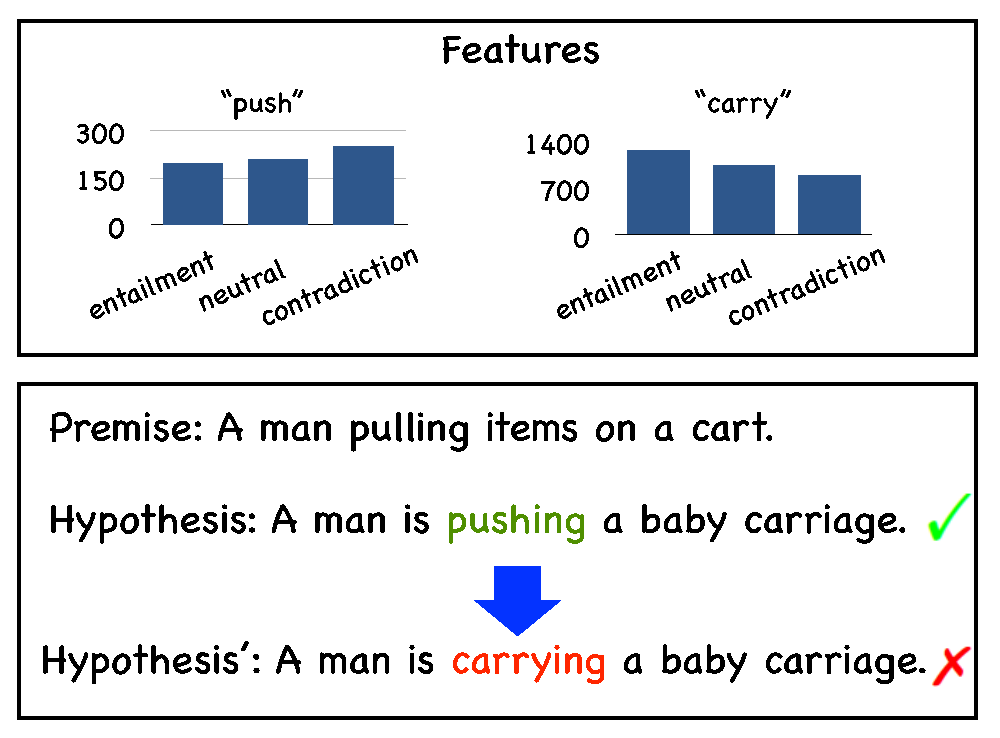
\includegraphics[angle=0]{figures/example.eps}}
% \caption{A real example of table linking. The red arrow points to the entity 
% predicted without using coherence feature, and the green arrow points to the entity
% predicted by using all features.}
% \label{fig:example}
% \end{figure}


\subsubsection{联合模型的作用}

这部分将验证整个联合模型框架的作用。
相对于联合模型计算整个输入表格与链接表格的相关度,
非联合模型中,单元格之间完全独立,各自计算字面描述与候选实体的匹配程度,
最后求平均得到整张表格上的相关度。
%受Sun等人\parencite{sun2015modeling}工作的启发,
我们将联合模型进行退化,
由于非联合模型仅考虑单个单元格,我们移除模型中的一致性特征模块,
并无需对不同单元格的特征输出求平均。
%Add formula if possible.
%which maximizes the margin between the gold entity $e^+$ and
%all the negative entities $e^-$ of the mention $x$.
%We investigate the effect of joint model without introducing the coherence feature.
%As discussed before, the cell and context features focus on relationships of individual mentions,
%then we simply transform the table linking problem into a traditional entity linking problem.
%%:given a mention's cell and context embedding (rather than a table of multiple mentions),link the mention to an entity in the knowledge base.Also, the gold linking result of a training table becomes a list of $(mention, entity)$ pairs.
%
%In this model,  $score(\cdot, \cdot)$ is similar with \eqnref{eqn:score},
%but remove the coherence feature, and don't need to average cell and context features over mentions.
%The parameter $\lambda$ is tuned in \{1.0, 2.0, 3.0, 4.0\}.
作为对比实验,我们同样从已有的联合模型中移除一致性特征,
并尝试分别使用RankNet模型或最大间隔损失(Max Margin)进行训练。

\begin{table}[ht]
    \centering
	\bicaption{不同模型训练方式在测试集上的跨语言链接准确率。}
    {Ablation test of train strategiess on validation set.}
    \label{tab:ablation-joint}
    \begin{tabular} {c|c|c|c}
        \hline
        Model       & Optimizer     & Coherence  &  Micro Acc.   \\
        \hline
        Non-Joint   & Max Margin    & N     & 0.586         \\
        Joint       & Max Margin    & N     & 0.574         \\
        Joint       & RankNet       & N     & 0.598         \\
        Joint       & RankNet       & Y     & 0.629         \\
        \hline
    \end{tabular}
\end{table}

\tabref{tab:ablation-joint}列出了这一部分实验在测试集上的微观准确率结果。
对比前两行结果,我们可以发现,若使用最大间隔损失,
非联合模型的效果反而优于联合模型。
主要原因有以下两点:
1) 非联合模型中,每一个单元格的多个负样本实体都能在训练过程中被利用,
而对于联合模型,由于负样本表格的生成依靠随机采样,并不是所有的负样本实体都会被使用;
2) 最大间隔损失侧重于正样本表格与不同负样本表格间的分值差距,
而对于不同错误程度的负样本表格之间,它们的偏序关系并没有被有效利用。
因此,相比于最大间隔损失,基于成对计算损失的RankNet更加适合于联合模型。
此外,在算法运行速度方面,非联合模型无需迭代预测步骤,因此显然比联合模型更高效。
而实验过程显示,联合模型平均只需要6轮迭代即可完成对每个测试表格的链接预测,
是一个可以被接受的运行速度。




\section{本章小结}

据我们所知,本章的工作是首次提出了在跨语言场景中进行互联网表格的实体链接问题。
为了使问题尽可能通用,本文研究在不利用任何非英文知识库作为过渡的情况下,
完成非英文表格到英文知识库(维基百科)的链接。
为此,本文提出了一个基于神经网络和跨语言词向量的链接模型,
并利用模型学习三种不同粒度的链接特征,
分别为单元格自身与目标实体的指示特征,单元格所在行列与目标实体的上下文特征,
以及同一列目标实体之间的一致性特征。
同时模型遵循联合训练框架,定义整张表格级别的链接匹配程度作为目标函数,
并使用迭代更新方式完成所有单元格的链接。
%To the best of our knowledge, this is the first piece of work that studies
%the cross-lingual entity linking problem for web tables. We proposed a neural
%network based joint model that takes advantage of features extracted from
%a cell, its context and semantic coherence within a table column. 
%versus a non-joint model that predicts the cells independently.
本文提出的模型在跨语言表格链接任务中取得了63\%的准确率,
考虑到此任务比单语言链接更具有挑战性,本文对后续的研究而言是一个良好的开端。
在不同设定上的多组对比实验显示,
三种粒度的特征对模型均起到明显效果,同时联合训练框架也具有实质性的帮助。
%Our best model achieves an accuracy of 63\%, for a task that is significantly more
%challenging than mono-lingual table linking.

后续的研究主要包括对表格中的单元格判断是否需要被链接,
本文的任务定义移除了这个问题带来的影响,
但显然,不可链接的单元格在互联网表格中也会普遍存在,
因此该研究具有其实际意义。
%Possible future work includes
%the automatic determination of whether a non-numerical string mention in 
%a cell should or should not be linked. We have ignored this problem in this
%paper but such un-linkable cells are abundant in web tables, too.


本章的研究成果已发表于2018年国际会议Thirty-Second AAAI Conference on Artificial Intelligence
(AAAI 2018),论文题目为``Cross-Lingual Entity Linking for Web Tables'' 。
